
%%%%%%%%%%%%%%%%%%%%%%%%%%%%%%%%%%%%%%%%%%%%%%%%%%%%%%%%%%%%%%%%%%%%%
%% This is a (brief) model paper using the achemso class
%% The document class accepts keyval options, which should include
%% the target journal and optionally the manuscript type.
%%%%%%%%%%%%%%%%%%%%%%%%%%%%%%%%%%%%%%%%%%%%%%%%%%%%%%%%%%%%%%%%%%%%%
\documentclass[journal=jacsat,manuscript=article]{achemso}

%%%%%%%%%%%%%%%%%%%%%%%%%%%%%%%%%%%%%%%%%%%%%%%%%%%%%%%%%%%%%%%%%%%%%
%% Place any additional packages needed here.  Only include packages
%% which are essential, to avoid problems later.
%%%%%%%%%%%%%%%%%%%%%%%%%%%%%%%%%%%%%%%%%%%%%%%%%%%%%%%%%%%%%%%%%%%%%
\usepackage{chemformula} % Formula subscripts using \ch{}
\usepackage[T1]{fontenc} % Use modern font encodings

%%%%%%%%%%%%%%%%%%%%%%%%%%%%%%%%%%%%%%%%%%%%%%%%%%%%%%%%%%%%%%%%%%%%%
%% If issues arise when submitting your manuscript, you may want to
%% un-comment the next line.  This provides information on the
%% version of every file you have used.
%%%%%%%%%%%%%%%%%%%%%%%%%%%%%%%%%%%%%%%%%%%%%%%%%%%%%%%%%%%%%%%%%%%%%
%%\listfiles

%%%%%%%%%%%%%%%%%%%%%%%%%%%%%%%%%%%%%%%%%%%%%%%%%%%%%%%%%%%%%%%%%%%%%
%% Place any additional macros here.  Please use \newcommand* where
%% possible, and avoid layout-changing macros (which are not used
%% when typesetting).
%%%%%%%%%%%%%%%%%%%%%%%%%%%%%%%%%%%%%%%%%%%%%%%%%%%%%%%%%%%%%%%%%%%%%
\newcommand*\mycommand[1]{\texttt{\emph{#1}}}

%%%%%%%%%%%%%%%%%%%%%%%%%%%%%%%%%%%%%%%%%%%%%%%%%%%%%%%%%%%%%%%%%%%%%
%% Meta-data block
%% ---------------
%% Each author should be given as a separate \author command.
%%
%% Corresponding authors should have an e-mail given after the author
%% name as an \email command. Phone and fax numbers can be given
%% using \phone and \fax, respectively; this information is optional.
%%
%% The affiliation of authors is given after the authors; each
%% \affiliation command applies to all preceding authors not already
%% assigned an affiliation.
%%
%% The affiliation takes an option argument for the short name.  This
%% will typically be something like "University of Somewhere".
%%
%% The \altaffiliation macro should be used for new address, etc.
%% On the other hand, \alsoaffiliation is used on a per author basis
%% when authors are associated with multiple institutions.
%%%%%%%%%%%%%%%%%%%%%%%%%%%%%%%%%%%%%%%%%%%%%%%%%%%%%%%%%%%%%%%%%%%%%
\author{Cong Wang}
\affiliation{College of Mathematics and Physics, Beijing University of Chemical Technology, Beijing 100029, China}
\altaffiliation{These authors contributed equally to this work}
\email{wangcongphysics@mail.buct.edu.cn}

\author{Pengzhi Wang}
\affiliation{GBA branch of Aerospace Information Research Institute, Chinese Academy of Sciences, Guangzhou 510700, China}
\alsoaffiliation{Key Laboratory of Luminescence and Optical Information, Ministry of education, Institute of Optoelectronic Technology, Beijing Jiaotong University, Beijing 100044, China}
\altaffiliation{These authors contributed equally to this work}

\author{Shengyao Chen}
\affiliation{CAS Center for Excellence in Nanoscience, National Center for Nanoscience and Technology, University of Chinese Academy of Sciences, Beijing 100190, China}

\author{Wen Wen}
\affiliation{CAS Center for Excellence in Nanoscience, National Center for Nanoscience and Technology, University of Chinese Academy of Sciences, Beijing 100190, China}

\author{Wenqi Xiong}
\affiliation{Key Laboratory of Artificial Micro- and Nano-structures of Ministry of Education and School of Physics and Technology, Wuhan University, Wuhan 430072, China}

\author{Zhenzhou Liu}
\affiliation{School of Physical Science and Technology, Inner Mongolia University, Inner Mongolia, Hohhot 010021, People’s Republic of China}

\author{Yifan Liu}
\affiliation{School of Physical Science and Technology, Inner Mongolia University, Inner Mongolia, Hohhot 010021, People’s Republic of China}

\author{Jiaqi He}
\affiliation{College of Mathematics and Physics, Beijing University of Chemical Technology, Beijing 100029, China}
\email{jqhe@mail.buct.edu.cn}

\author{Yongsheng Wang}
\affiliation{Key Laboratory of Luminescence and Optical Information, Ministry of education, Institute of Optoelectronic Technology, Beijing Jiaotong University, Beijing 100044, China}
%%%%%%%%%%%%%%%%%%%%%%%%%%%%%%%%%%%%%%%%%%%%%%%%%%%%%%%%%%%%%%%%%%%%%
%% The document title should be given as usual. Some journals require
%% a running title from the author: this should be supplied as an
%% optional argument to \title.
%%%%%%%%%%%%%%%%%%%%%%%%%%%%%%%%%%%%%%%%%%%%%%%%%%%%%%%%%%%%%%%%%%%%%
\title[An \textsf{achemso} demo]
  {Anisotropic Properties of Tellurium Nanoflakes Probed by Polarized Raman and Transient Absorption Microscopy: Implications for Polarization-sensitive Applications}

%%%%%%%%%%%%%%%%%%%%%%%%%%%%%%%%%%%%%%%%%%%%%%%%%%%%%%%%%%%%%%%%%%%%%
%% Some journals require a list of abbreviations or keywords to be
%% supplied. These should be set up here, and will be printed after
%% the title and author information, if needed.
%%%%%%%%%%%%%%%%%%%%%%%%%%%%%%%%%%%%%%%%%%%%%%%%%%%%%%%%%%%%%%%%%%%%%
%\abbreviations{IR,NMR,UV}
%\keywords{anisotropic properties, tellurium nanoflakes, density functional theory, polarized raman spectrums, transient absorption microscopy}

%%%%%%%%%%%%%%%%%%%%%%%%%%%%%%%%%%%%%%%%%%%%%%%%%%%%%%%%%%%%%%%%%%%%%
%% The manuscript does not need to include \maketitle, which is
%% executed automatically.
%%%%%%%%%%%%%%%%%%%%%%%%%%%%%%%%%%%%%%%%%%%%%%%%%%%%%%%%%%%%%%%%%%%%%
\begin{document}

%%%%%%%%%%%%%%%%%%%%%%%%%%%%%%%%%%%%%%%%%%%%%%%%%%%%%%%%%%%%%%%%%%%%%
%% The "tocentry" environment can be used to create an entry for the
%% graphical table of contents. It is given here as some journals
%% require that it is printed as part of the abstract page. It will
%% be automatically moved as appropriate.
%%%%%%%%%%%%%%%%%%%%%%%%%%%%%%%%%%%%%%%%%%%%%%%%%%%%%%%%%%%%%%%%%%%%%
\begin{tocentry}
\centering
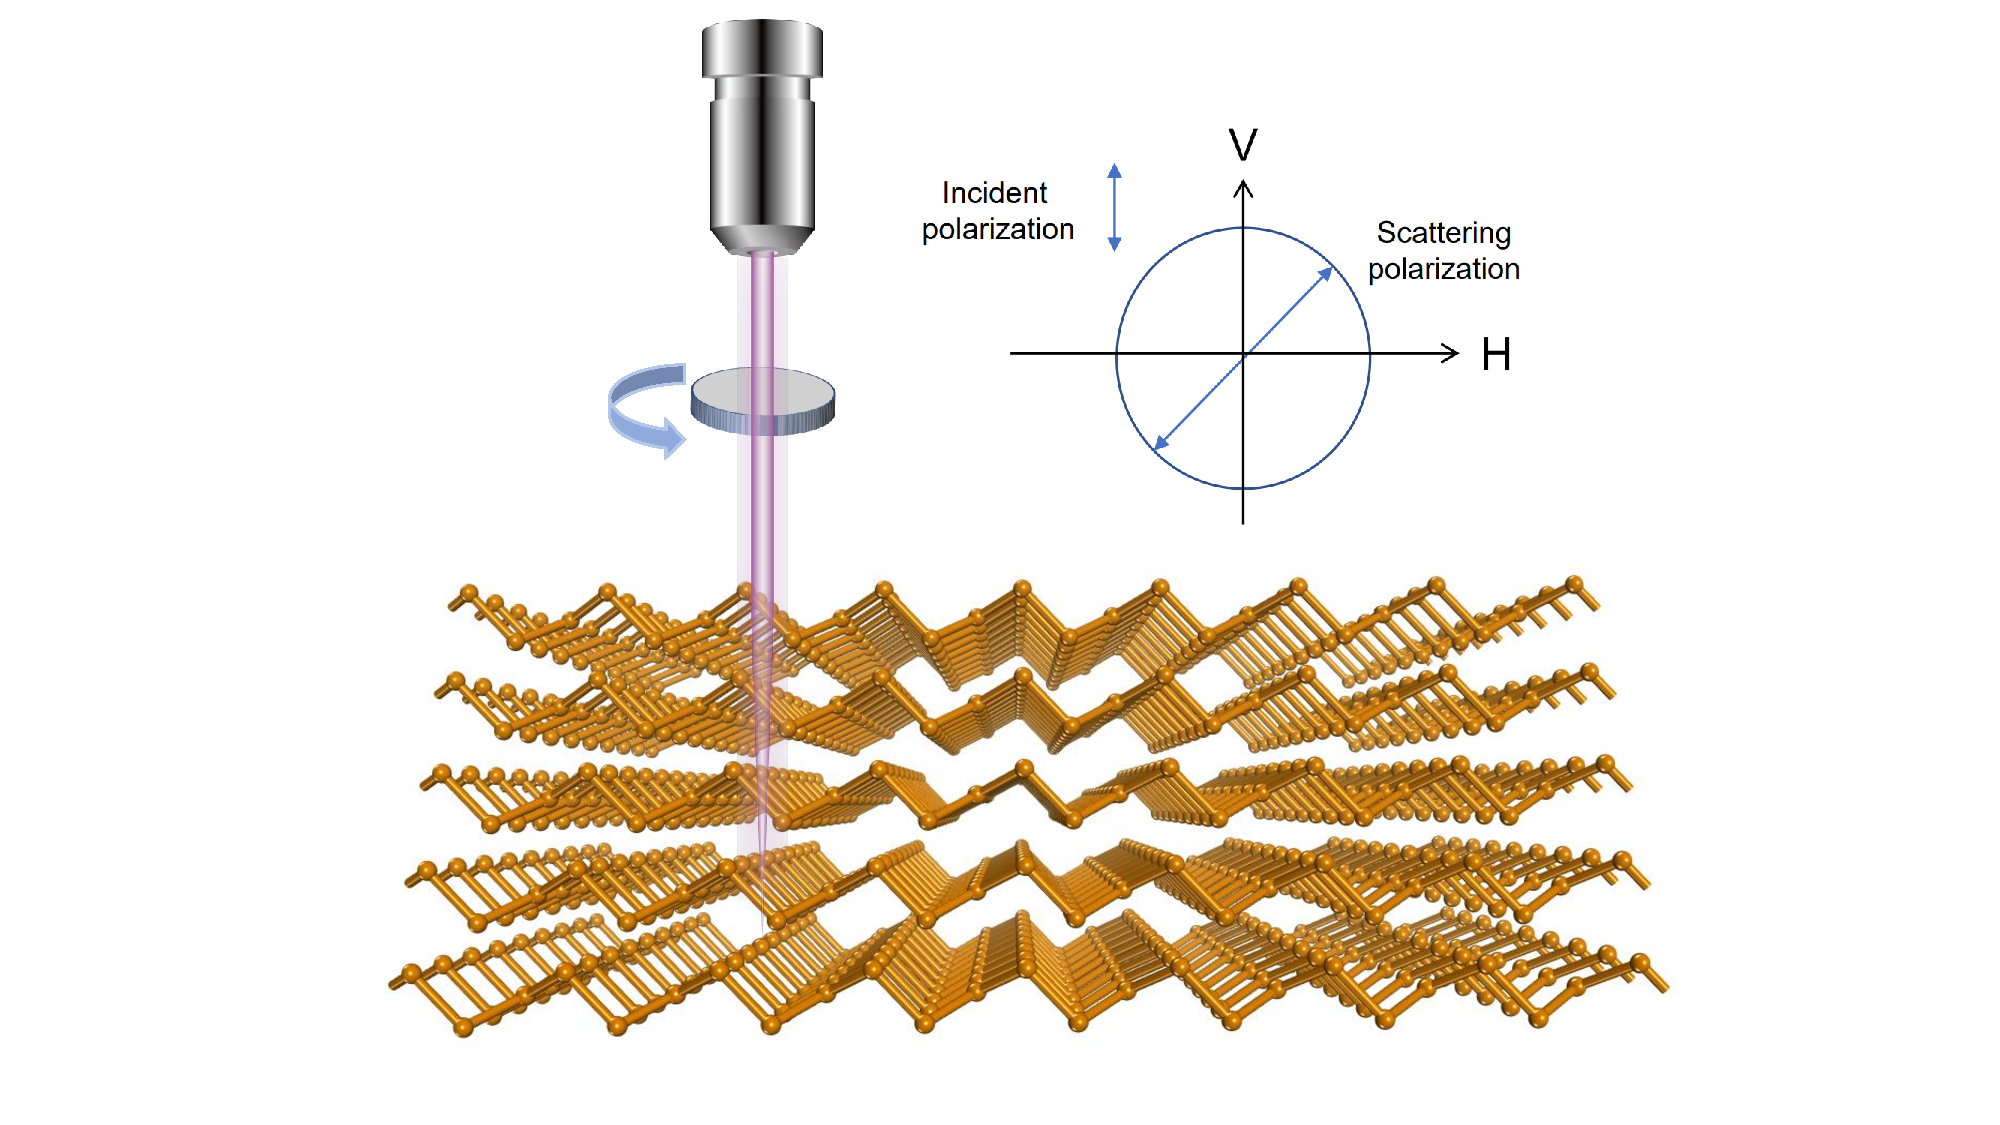
\includegraphics[height=4.45cm]{TOC.pdf}
\end{tocentry}

%%%%%%%%%%%%%%%%%%%%%%%%%%%%%%%%%%%%%%%%%%%%%%%%%%%%%%%%%%%%%%%%%%%%%
%% The abstract environment will automatically gobble the contents
%% if an abstract is not used by the target journal.
%%%%%%%%%%%%%%%%%%%%%%%%%%%%%%%%%%%%%%%%%%%%%%%%%%%%%%%%%%%%%%%%%%%%%
\begin{abstract}
  Recently, two-dimensional (2D) elemental materials tellurium (Te) has drawn considerable attention since it possesses high transport properties, wide broadband absorption, excellent thermoelectric properties and prominent air stability. Yet, anisotropic properties and carrier dynamincs of this material are less stated. Here, Te nanoflakes are prepared by hydrothermal method. Highly anisotropic properties are illustrated by polarized raman spectrums and transient absorption spectroscopic measurements as well as density functional theory (DFT) calculation. Photocarrier dynamincs are probed by temporally resolved transient measurements with an exciton lifetime of 25 ps. These results imply that Te can be treated as a competitive material for further anisotropic devices and applications.
\end{abstract}

\textbf{Keywords:} anisotropic properties, tellurium nanoflakes, density functional theory, polarized raman spectrums, transient absorption microscopy.

%%%%%%%%%%%%%%%%%%%%%%%%%%%%%%%%%%%%%%%%%%%%%%%%%%%%%%%%%%%%%%%%%%%%%
%% Start the main part of the manuscript here.
%%%%%%%%%%%%%%%%%%%%%%%%%%%%%%%%%%%%%%%%%%%%%%%%%%%%%%%%%%%%%%%%%%%%%
\section{Introduction}
The fact that graphene was discovered triggered intense attention in exploring the properties of two dimension (2D) materials\cite{novoselov2004electric} including hexagonal boron nitride (hBN)\cite{song2010large}, transition metal
dichalcogenides (TMDs)\cite{wang2012electronics}, perovskite\cite{RicciardulliEmergingperovskitemonolayers2021} and transition metal oxides\cite{kalantar2016two}. However, elemental 2D materials are quite rare. In fact, there are less than 20 types of them\cite{cai2020tellurene}, including graphene, silicene\cite{vogt2012silicene}, phosphorene\cite{liu2014phosphorene}, etc. 2D Te, or tellurene, is predicted by theoretical calculations and proved by experiments, as the first elemental materials in group-VIA. Although it is more likely to form one-dimensional structure of Te crystal due to its chain-like arrangement, the first attempt of 2D hexagonal Te was successfully made in 2014\cite{wang2014van}. The nanoplate was obtained on soft mica layers via epitaxy method. So far, monolayer and few-layer Te nanofalkes can be fabricated by several strategies, such as physical vapor deposition (PVD)\cite{yang2018highly,zhao2020evaporated}, liquid phase exfoliation\cite{xie2018ultrathin} and hydrothermal synthesis\cite{amani2018solution,gao2019one,lono2021local}.

With improving synthesis methods, some literatures on physical properties of 2D Te have been established and drawn considerable attention. Because of its unique properties, like high carrier mobility\cite{qiu2018quantum}, prominent air stability\cite{li2021bilayer}, wide broadband absorption\cite{zhang2019broadband} and  excellent thermoelectric transport properties\cite{peng2015anisotropic,peng2014elemental}, 2D Te has a great perspective in various devices and applications\cite{shi2020two}. Nowadays, multiple researches have showed integration of 2D Te in versatile devices and applications with high performance, including photodetectors\cite{wang2014van,amani2018solution,tong2020stable,shen2019tellurene,deckoff2019tellurene}, field-effect transistors\cite{jiang2021end,zhao2020evaporated,wang2018field,ren2019gate}, lasers\cite{zhang2020passively}, gas sensors\cite{xu2021gas,wang2018effects,cui2020tellurene}, chemical sensors\cite{wang2018effects,wang2019tellurene} and biosensors\cite{guo2020tellurene}. Strong nonlinear optical responses of Te illustrates its potential applications for nonlinear photonics and optoelectronic devices\cite{wu20192d}. Besides, combining Te with other materials, such as Te/PVP membranes\cite{guo2019two} and Te@Se roll-to-roll nanotubes\cite{huang2019enhanced}, further improves the performance of practical applications. However, anisotropic devices based on 2D materials are rarely developed\cite{xin2020polarization,yuan2015polarization}, more attempts should be made to embrace the unique properties. 

Here, we conduct a theoretical and experimental work on the anisotropic properties of Te nanoflake obtained by hydrothermal method. From DFT calculations, the effective mass of carriers along different direction suggests anisotropism of Te crystal, which has been further confirmed by polarized raman spectrums and transient absorption spectroscopic measurements with 2-fold symmetry. The results are consistent with theory. Besides, photocarrier dynamics of Te nanoflakes are also established, with exciton lifetime of 25 ps obtained by temporally resolved transient measurements. These results provide basic understanding for implementing tellurium in various anisotropic optoelectronic devices. The performance of photodetectors based on this characteristic can be largely improved with  higher photoconductive sensitivity and responsivity under precise regulation.


\section{Results and discussion}
Te nanosheets are synthesized by hydrothermal method, as shown in Fig. 1(a). Via scanning electron microscope (SEM) characterization, a regular and complete morphology of sample are observed (Fig. 1(b)). To figure out the composition of the Te nanosheets, we perform energy dispersive spectrometer (EDS) characterization on one of the Te nanosheets (Fig. 1(c)). The result shows that the sample is not doped with other elements, as shown in Fig. 1(d). Besides, we utilize TEM characterization to further confirm that the synthesized nanosheets contain only Te element (Fig. 1(e), (f)). Fig. 1(g) shows high-quality Te crystals  are analyzed by the high-angle annular dark-field scanning transmission electron microscopy (HAADF–STEM). Structural and material characterization of Te nanosheets indicates its high quality, which is appropriate to polarized raman spectrums and transient absorption spectroscopic measurements.

\begin{figure}
  \centering
  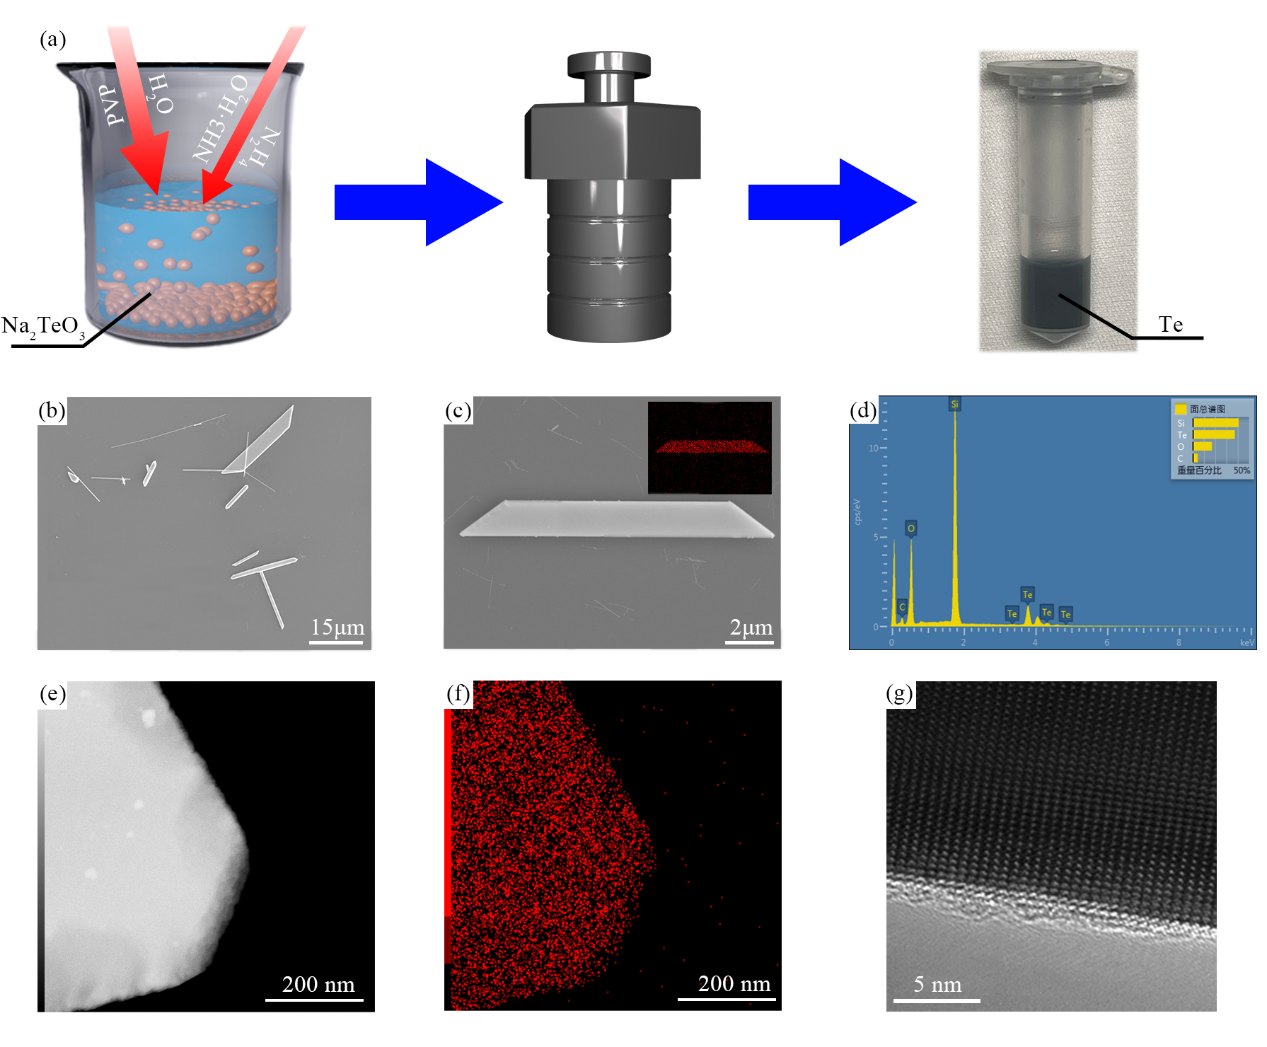
\includegraphics[width=\linewidth]{method.png}
  \caption{Hydrothermal growth of Te nanosheets and material characterization (a) Schematic diagram of hydrothermal synthesis of Te nanosheets. (b) SEM image of Te nanosheets synthesized by hydrothermal method. (c) SEM image of a single Te nanosheet. The inset shows EDS map of the sample. (d) The EDS analysis of the Te sample in (c). (e-g) TEM image, EDS map and HAADF–STEM image of the Te nanosheets.}
    \label{fig:method}
\end{figure}

A software called Vesta is used to establish the atomic structure model of Te crystal, as shown in Fig. 2(a)-(c). Since single Te atom is only covalently bonded to the the two nearest neighbor Te atoms,  a triangular helix chain is formed of Te atoms, which makes Te is actually a 1D structure instead of a 2D van der Waals system. The chains are arranged in a hexagonal pattern which indicates its anisotropic properties. In fact, the zigzag direction is easily observed from the c-axis.

\begin{figure}
  \centering
  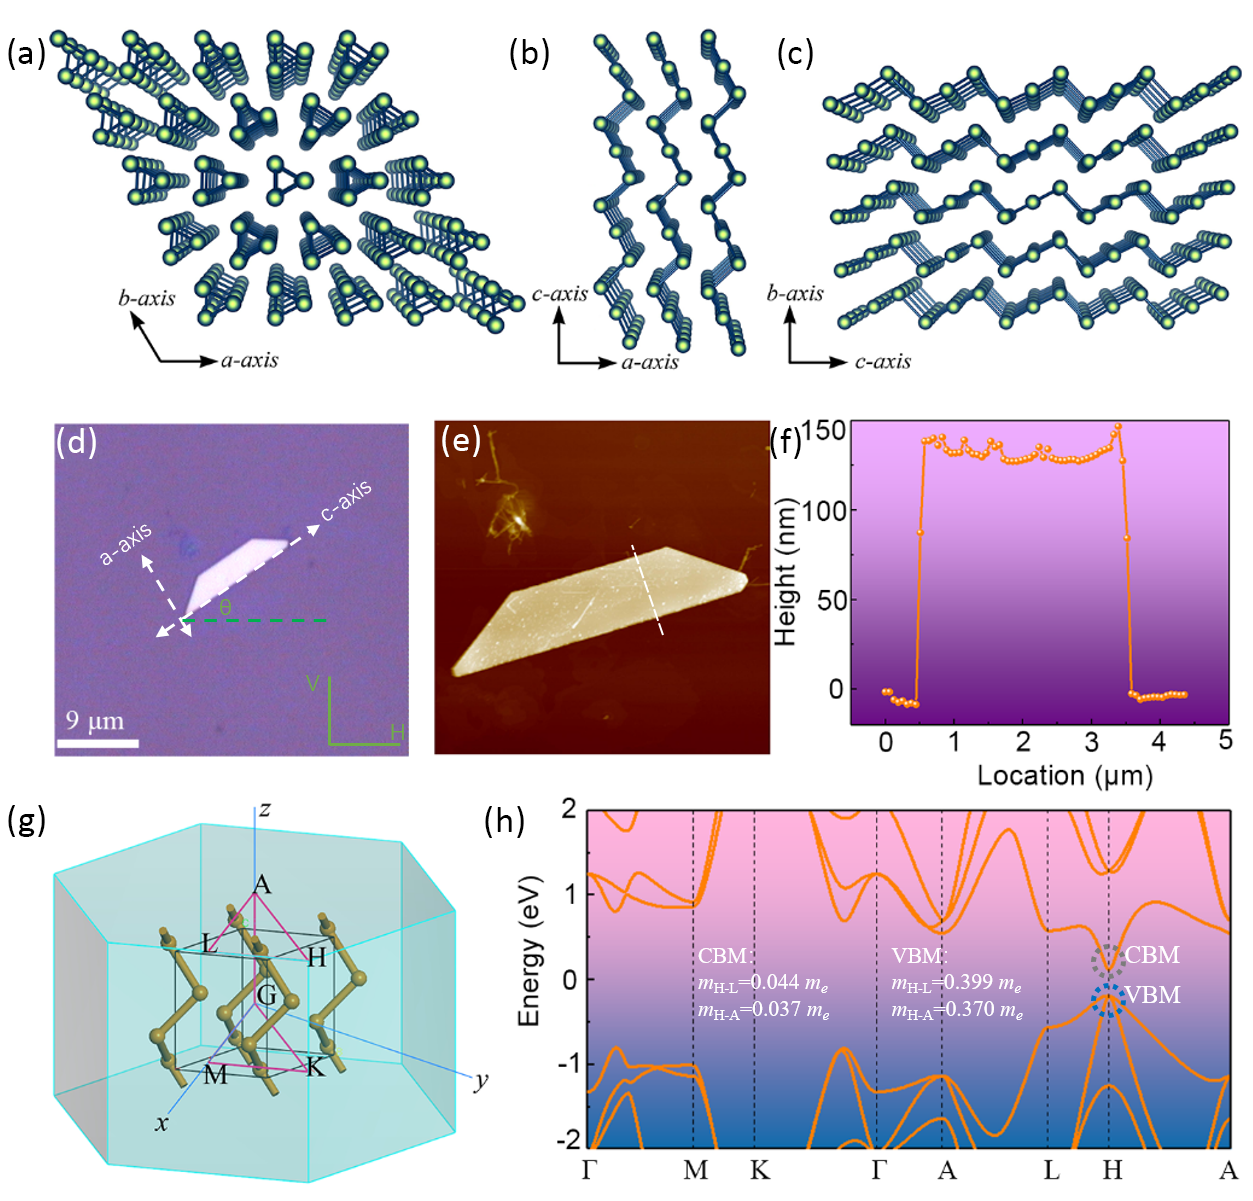
\includegraphics[width=\linewidth]{AFM.png}
  \caption{Characterzation of Te nanoflake sample and DFT study. (a)-(c) Atomic structure of few-layer Te from top view and side view.  (d) Optical mircoscope image of Te nanoflake sample. (e) Same image under atomic force microscope as (d) and (f) the line profile of the thickness of the sample. (g) The Brillouin zone of  Te with high-symmetry k-ponits labeled. (h) The bandstructure calculated by DFT method as well as the effective mass of electron and hole along the direction H-L and H-A.}
    \label{fig:AFM}
\end{figure}

To characterize our sample, Te nanofalkes were obtained and transferred to a Si substrate on the top of a SiO$_2$ wafer. The optical microscope image (Fig. 2(d)) illustrated that Te nanoflake froms a trapezoid shape, with a length of about 7 to 14 micrometer, and a width of around 3 micrometer. An atomic force microscope (AFM) image (Fig. 2(e)) of same Te nanoflake illustrates a thickness of 120 nm from the AFM height profile shown in Fig. 2(f). 

The electronic band structure of few-layer Te has been further discussed by density functional theory (DFT) method. The Brillouin zone is shown in Fig. 2(g), as well as the labeled high-symmetry k-ponits. From the performed calculation, a direct bandgap of ~0.35 eV is obtained at H point in Fig. 2(h). Also, the effective masses of charged carriers are calculated. Although little difference is shown for effective mass of holes around VBM, there is a significant difference about 20\% for electons around CBM along H-L (0.044 $m_e$) and H-A (0.037 $m_e$) directions, which suggests the existence of anisotropic properties in Te crystal. Here, $m_e$ is electron rest mass.  

\begin{figure}
  \centering
  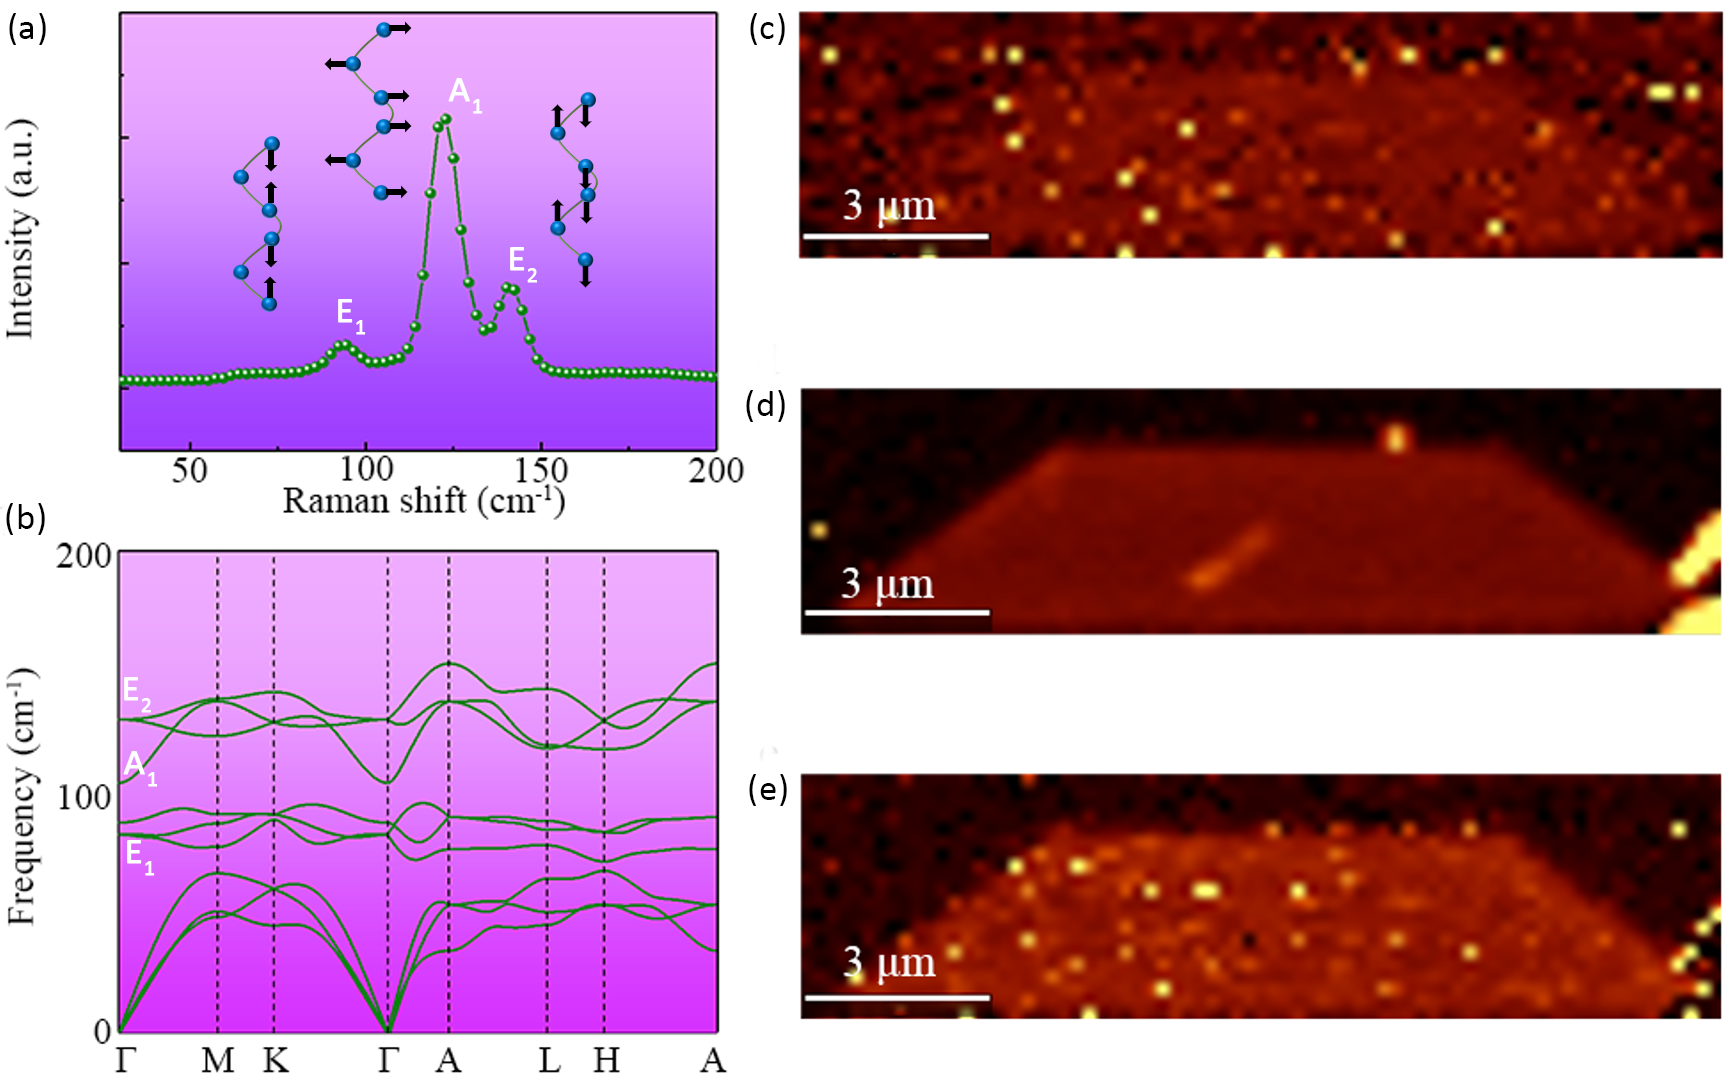
\includegraphics[width=\linewidth]{raman.png}
  \caption{Raman spectrums with map scans of each peak and calculated phonon dispersion. (a) Raman spectra of tellurene nanoflake sample. (b) Phonon dispersion calculated by DFT method. (c)-(e) Raman peak intensity mappings of E$_1$, A$_1$ and E$_2$ of Te nanoflake sample,respectively.}
    \label{fig:raman}
\end{figure}

A more detailed study of this Te nanoflake sample is further conducted by raman techniques. Raman spectroscopy in Fig. 3(a) shows Te nanoflake has three active raman phonon modes. Besides, phonon dispersion is calculated by DFT method (see Fig. 3(b)), including the acoustic and optical branches. Due to the absence of spin-orbit coupling, the low-frequency optical branches E$_1$ (bond bending vibration) at 104 cm$^{-1}$, high-frequency optical branches A$_1$ (bond breathing mode) at 82 cm$^{-1}$ and E$_2$ (bond stretching mode) at 130 cm$^{-1}$ are slightly lower than our Raman scattering results where three vibration modes are at 122 cm$^{-1}$, 94 cm$^{-1}$ and 142 cm$^{-1}$ (see Fig. 3(a)), respectively. Since higher frequency optical phonons are frequently demonstrated by raman scattering, results from both DFT theory and raman measurements are compared. Obviously, the theoretical values of three higher optical branches are sightly smaller than the measured values. which can be attributed to the fact that GGA underbinds and lattice constants overestimation\cite{peng2015anisotropic}. A bandgap of about 10 cm$^{-1}$ occurs between the lower and higher optical branches, due to the interaction between covalent bonding, which links to A$_1$ and E$_2$ modes, and van der Waals bonding, which is related to E$_1$ mode in Te\cite{martin1976intermolecular}.  Finally, the raman peak intensity mappings of E$_1$, A$_1$ and E$_2$ from Te nanoflake sample are shown in Fig. 3(c)-(e) respectively, which are quite uniform, confirming the fine crystalline quality of Te nanoflake sample.
\begin{figure}
  \centering
  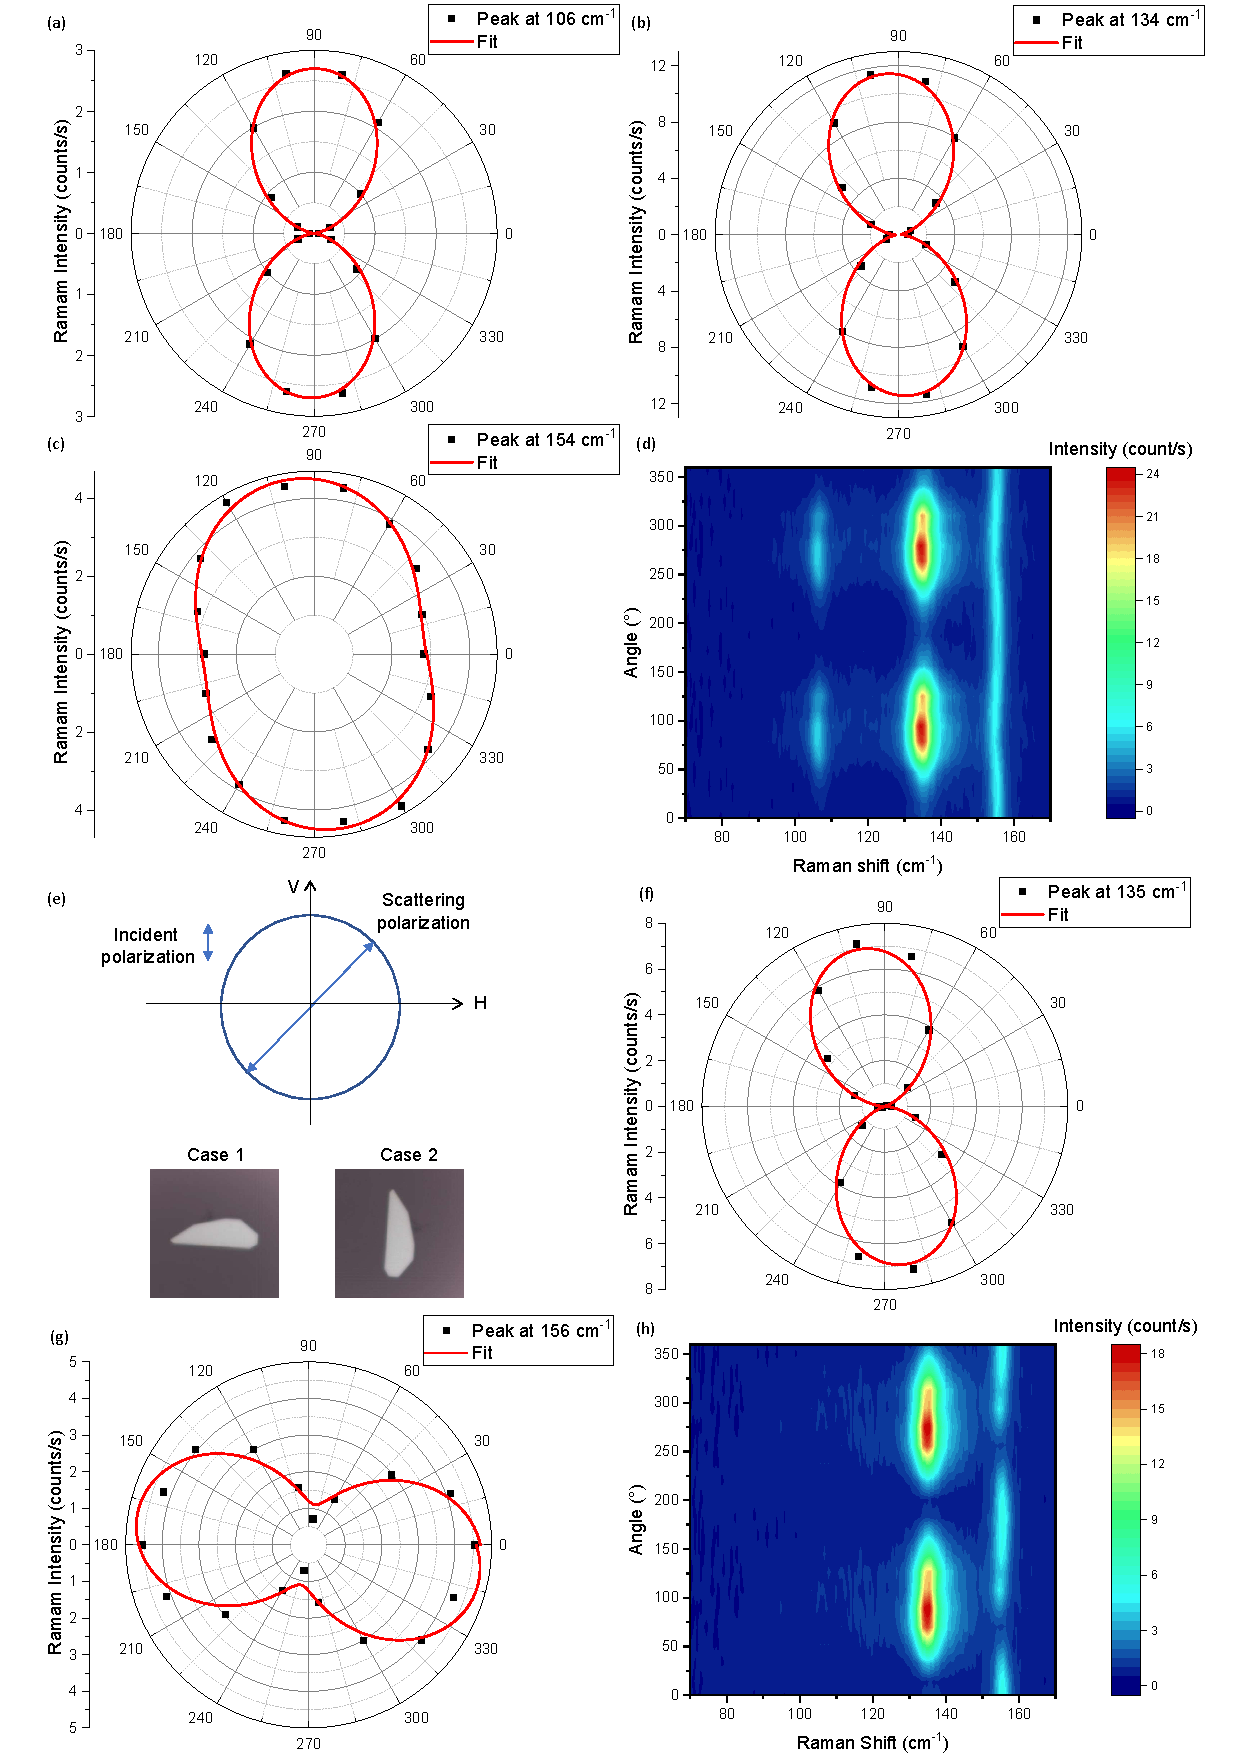
\includegraphics[width=13cm]{PR1.pdf}
  \caption{Polarized raman spectroscopy. (a)-(c) The raman peak intensity as a function of rotating angle at E$_1$, A$_1$, E$_2$ modes obtained from case 1, respectively. (d) Raman profile the polarized raman intensity mapping as a function of raman shift and scattering angle of case 1. (e) Raman setup in our lab configuration. (f),(g) The raman peak intensity as a function of rotating angle at A$_1$, E$_2$ modes obtained from case 2, respectively. (h) Same as (d), but obtained from case 2.}
    \label{fig:PR}
\end{figure}

To illustrate the anistropic properties of the Te nanoflakes, the polarized raman spectrums are measured and the results are summarized in Fig. 4. The incident laser is linear polarized along vertical (V) direction in the lab configuration. Instead of rotating the Te nanoflake sample, a linear polarizer is put in the reflected arm, so that the collected scattering signals are also polarized and the polarization direction can be determined  by simply rotating the polarizer. According to Raman tensor theory, the scattered raman intensity can be calculated by following equation\cite{kranert2016raman}:

\begin{equation}
I = \left|e_{\mathrm{i}} \cdot \mathbf{R} \cdot e_{\mathrm{s}}\right|^{2}
\end{equation}
where $e_{\mathrm{i}}$ and $e_{\mathrm{s}}$ are the incident and scattering polarization vector, respectively. $\mathbf{R}$ is the raman tensors of each mode\cite{tong2020stable}, which is 3 $\times$ 3 matrix with several parameters from a to h, which are determined by crystal symmetry\cite{pine1971raman}. In our experiment, the sample is placed in two different ways according to the direction of long edge. One is along H direction,  $e_{\mathrm{i}}$=[1, 0, 0], $e_{\mathrm{s}}$=[$\sin \theta$, 0, $\cos \theta$], where $\theta$ is the angle between the long edge of Te nanoflake and incident and scattering polarization; the other is along V direction, $e_{\mathrm{i}}$=[0, 0, 1], $e_{\mathrm{s}}$=[$\cos \theta$, 0, $\sin \theta$]. Finally, we can easily obtain the angle dependence of raman intensity. For the former, the three modes are:
\begin{equation}
I_{E_{1}} = \left|\left.[1, 0, 0]\left[\begin{array}{ccc}
a & 0 & 0 \\
0 & b & c \\
0 & c & 0
\end{array}\right]\left[\begin{array}{c}
\sin \theta \\
0 \\
\cos \theta
\end{array}\right]\right|^{2} = \left|a \sin \theta\right|^{2},\right.
\end{equation}

\begin{equation}
I_{A_{1}} = \left|\left.[1, 0, 0]\left[\begin{array}{ccc}
d & 0 & 0 \\
0 & e & 0 \\
0 & 0 & f
\end{array}\right]\left[\begin{array}{c}
\sin \theta \\
0 \\
\cos \theta
\end{array}\right]\right|^{2} = \left|d \sin \theta\right|^{2},\right.
\end{equation}

\begin{equation}
I_{E_{2}} = \left|\left.[1, 0, 0]\left[\begin{array}{ccc}
0 & g & h \\
g & 0 & 0 \\
h & 0 & 0
\end{array}\right]\left[\begin{array}{c}
\sin \theta \\
0 \\
\cos \theta
\end{array}\right]\right|^{2} = \left|h \cos \theta\right|^{2};\right.
\end{equation}

For the latter, we have:
\begin{equation}
I_{E_{1}} = \left|\left.[0, 0, 1]\left[\begin{array}{ccc}
a & 0 & 0 \\
0 & b & c \\
0 & c & 0
\end{array}\right]\left[\begin{array}{c}
\cos \theta \\
0 \\
\sin \theta
\end{array}\right]\right|^{2} = 0,\right.
\end{equation}

\begin{equation}
I_{A_{1}} = \left|\left.[0, 0, 1]\left[\begin{array}{ccc}
d & 0 & 0 \\
0 & e & 0 \\
0 & 0 & f
\end{array}\right]\left[\begin{array}{c}
\cos \theta \\
0 \\
\sin \theta
\end{array}\right]\right|^{2} = \left|f \sin \theta\right|^{2},\right.
\end{equation}

\begin{equation}
I_{E_{2}} = \left|\left.[0, 0, 1]\left[\begin{array}{ccc}
0 & g & h \\
g & 0 & 0 \\
h & 0 & 0
\end{array}\right]\left[\begin{array}{c}
\cos \theta \\
0 \\
\sin \theta
\end{array}\right]\right|^{2} = \left|h \cos \theta\right|^{2}.\right.
\end{equation}
The results of polarized raman spectrums are illustrated in Fig. 4(a)-(c) for former case with E$_1$, A$_1$, E$_2$ modes and (f) (g) for latter case with A$_1$, E$_2$ modes, respectively. Comparing the experiment data, most results can be fitted quite well. However, the behaviors of raman peak at around 155 cm$^{-1}$ in both cases are not as expected, and the fitting curve is not even closed for the latter. This phenomenon can be attributed to that E$_1$ mode also contributes to this raman peak as well as the E$_2$ mode. Some previous works also mentioned this problem\cite{tong2020stable,qin2020raman}. However, further theory should be developed to figure this phenomenon out. Besides, the polarized raman intensity mappings of Te nanoflake for both situations as a function of raman shift and scattering angle are aslo summarized in Fig. 4(d) and (h) for both cases, respectively.     

We then studied the Te nanoflake sample with transient absorption (TA) method, which the pump and probe pulses are selected to be linearly polarized along V and H directions in the lab configuration, respectively (see Fig. 2(d). In our transient measurements, as mentioned in experimental part, a 620 nm pump pulse injects electron-hole pairs to the Te nanoflake sample. The peak fluence of pump beam is about 37.2 $\mu$J/cm$^2$. Then the time evolution of injected photocarriers are observed by measuring the differential reflection ($\Delta$R), which is defined as the pump-induced relatived change of the probe reflection (the 820 nm probe pulses). As shown in Fig. 5(a), there is relatively small background before the zero probe delay. Then the $\Delta$R signal ascend a peak rapidly near the zero position, after that the signal decays exponentially, which is demonstrated in Fig. 5(b), the exact same signal as the one showed in Fig. 5(a), but for a quite long time scale. A fit from the peak to about 140 ps is illustrated with red solid curve by two exponential decay function, $\Delta R/R_0= A_0 +A_1 e^{t/\tau_1}+A_2 e^{t/\tau_2}$. The smaller time constant ($\tau_1$) which is about 2.5 ps, is attributed to the processes associated with thermal relaxation and exciton formation. And the larger time constant ($\tau_2$) of about 23.6 ps can be treated as the lifetime of excitons in  Te sample. Since the energy of pump pulses (2 eV) and probe pulses (1.51 eV) are much higher than the bandgap of Te (0.31 eV from DFT calculation), the fast process governs majority of time evolution, that is, A$_1$/A$_2$ = 7.4. Also, there is a quite long process, which is more than 1 ns, could be attributed to the photocarriers trapped at defect states. Fig. 5(c) summarizes differential reflection signals at 2 ps as a function of different pump fluences. The red solid line is the linear fit, which suggests that  no saturation is found during our measurements.

Since single Te crystal has the trigonal space group of D$_3$, anisotropic properties should be presented. In other words, it is quite necessary to study the relation between crystal symmetry and $\Delta$R signals. Fig. 5(d) shows the peak $\Delta$R signal as a function of the sample direction  $\theta$. The results are obtained by rotating the sample on a homemade stage. Clearly, a pronounced angular dependence is shown here. The maximum and minimum values are obtained when $\theta$ equals 90 degree and 0 degree, respectively. Although angular dependence of $\Delta$R signals is quite obvious, their time delay remains independent. That is, there is no extra carrier dynamic process caused anisotropic properties of Te. The red solid curve is the fit by sine-squared function, which is consistent with the results we obtain from polarized raman measurements.  

\begin{figure}
  \centering
  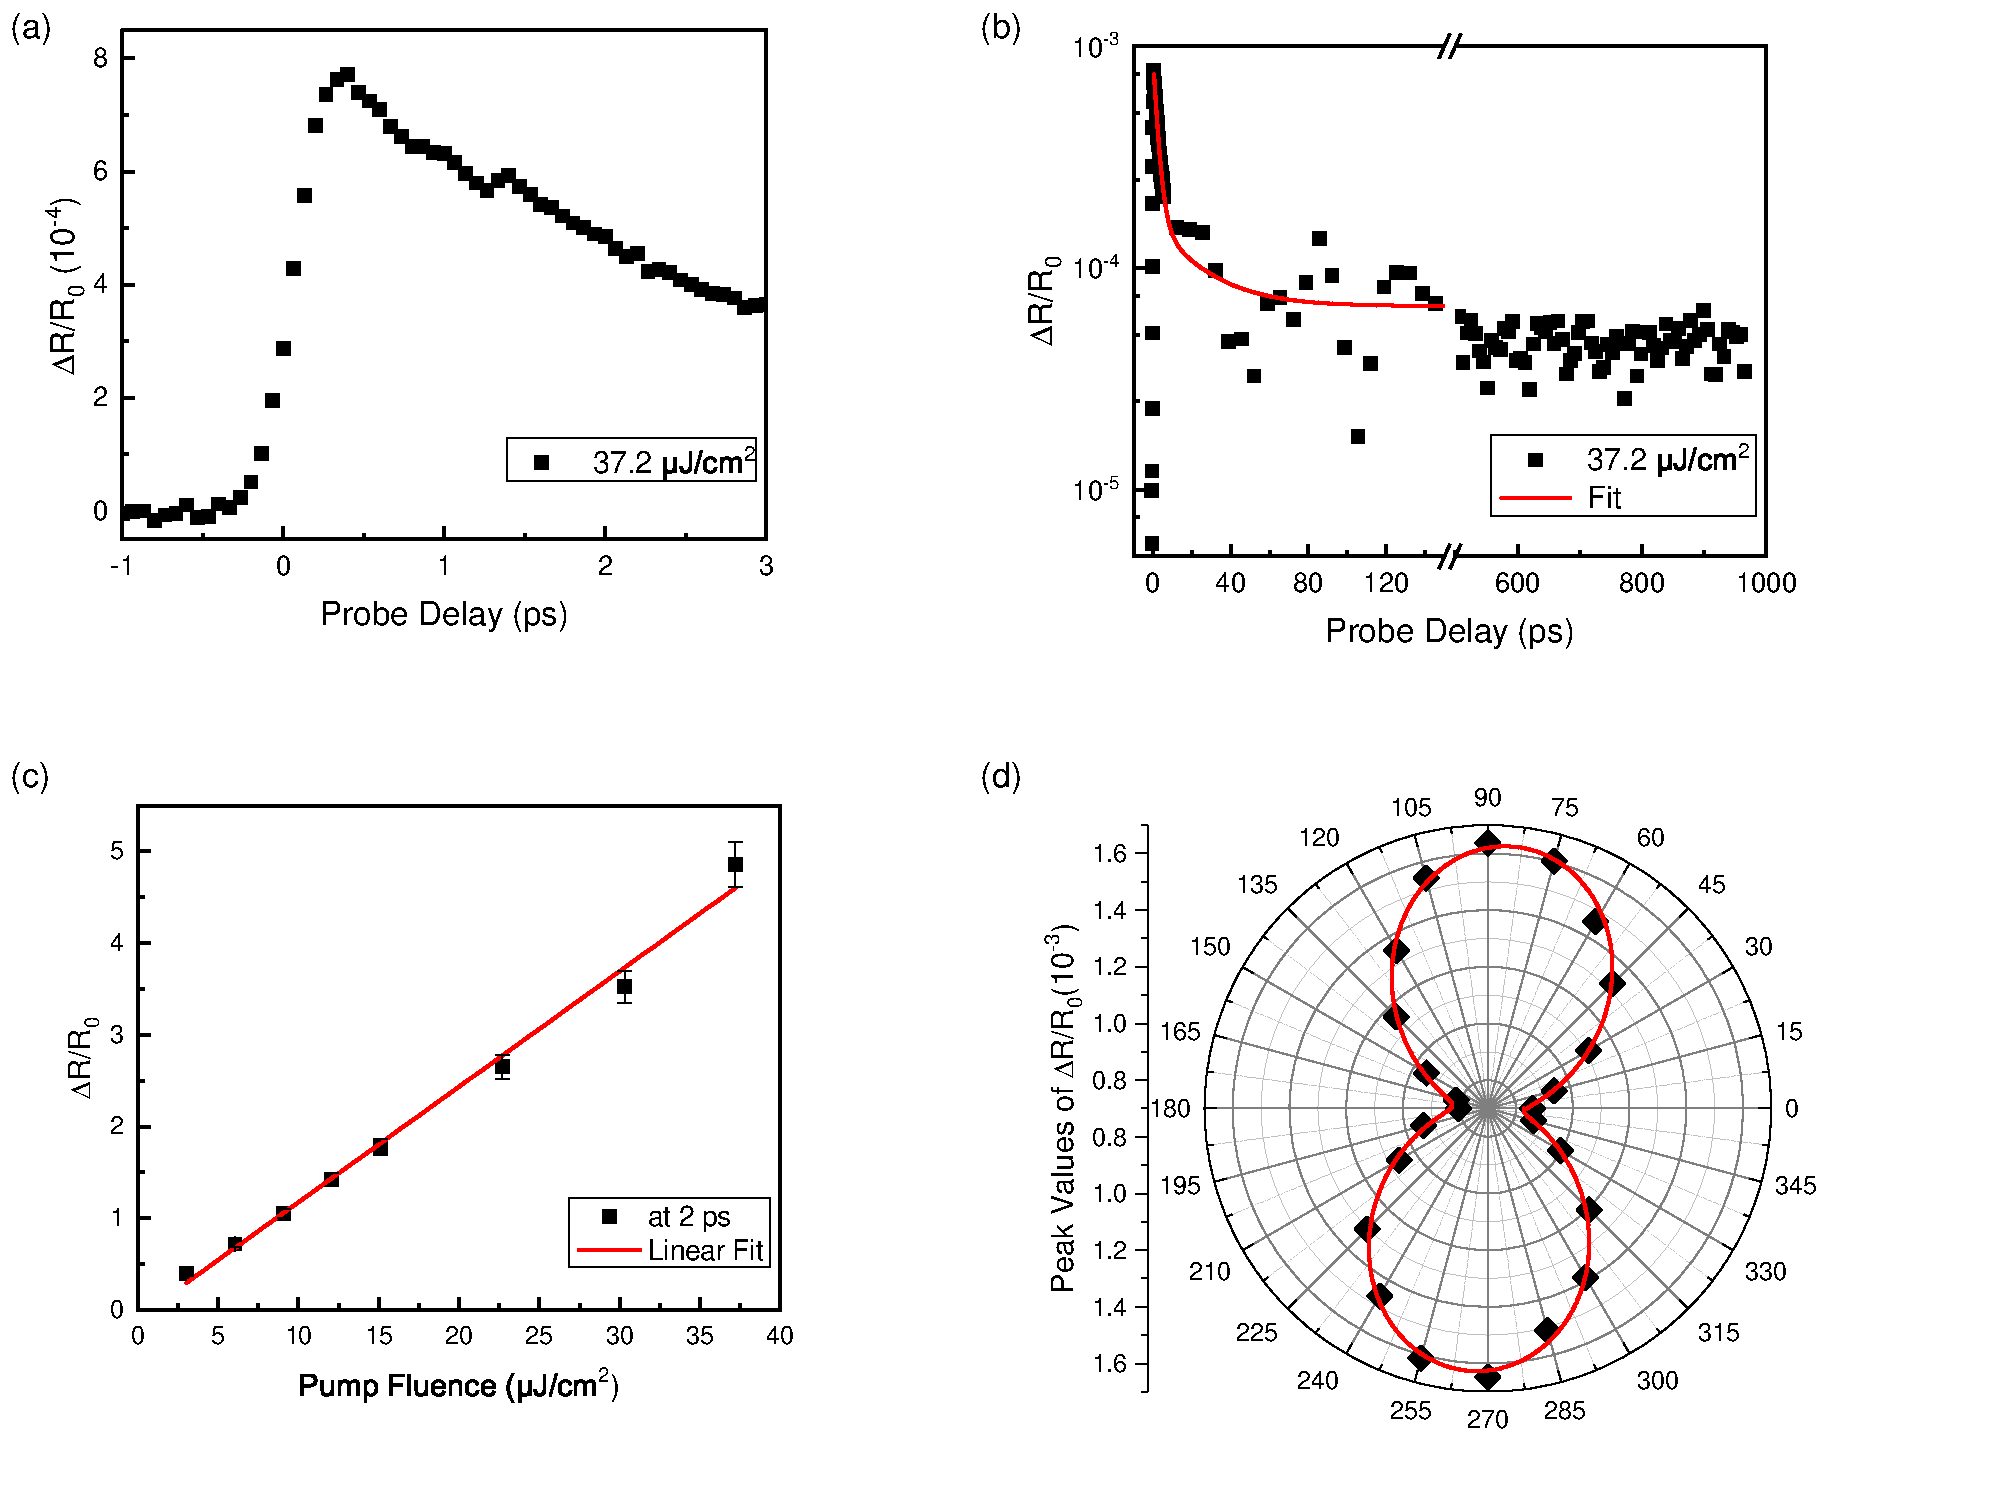
\includegraphics[width=\linewidth]{TA.pdf}
  \caption{Time-resolved differential reflection signal and angular dependence from the Te nanoflake sample. (a) Differential reflection signals measured from Te sample with pump fluence of 37.2 $\mu J/cm^2$. (b) The same process of (a), but for a long time range. (c) Differential reflection signals at 2 ps as a function of pump fluence. (d) The peak differential reflection signals as a function of $\theta$, the angle between the long edge of the flake and the horizontal direction in the lab configuration. The red solid curve is the fit by sine-sqaured function.}
    \label{fig:TA}
\end{figure}

\section{Conclusions}
We fabricated Te nanoflakes via hydrothermal method, and their qualities have been confirmed with raman map. The anisotropic properties of this material in optical response and carrier dynamics have been predicted by first-principle calculations, and further been confirmed with optical measurements, including polarized raman spectrums and transient absorption spectroscopic measurements. Besides, dynamics of photocarries are studied with an lifetime of 25 ps. With these results, tellurium may play a significant role as a promising layered material for developing  anisotropic devices, such as polarization-sensitive photodetectors, and also be integrated with other 2D materials for buliding novel van der Waals structures and applications.

\section{Experimental}

\subsection{Sample Preparation}
Tellurium nanoflakes were prepared by a revised hydrothermal method. Na$_2$TeO$_3$ was reducted with N$_2$H$_4$ in the alkaline solution of polyvinylpyrrolidone (PVP). Then the Te nanoflakes solution was diluted with anhydrous ethanol and dropped onto the SiO$_2$/Si substrate. 

\subsection{Atomic Force Microscopy and Polarazied Raman Spectroscopy}
AFM images are measured by using Bruker Multimode 8HR in the tapping mode.

Raman spectrums are conducted by LABRAM ARAMIS system (Horiba). The incident laser is about 532 nm with 1/10 total power , and scattering signals are reflected to the detector.

Polarized Raman spectrums are also conducted by same system. As mentioned, the polarization directions of the incident laser is always along vertical direction (V) in the lab configuration, shown in Fig. 2(d) and the scattering signal are measured by a polarizer. Each step is about 20 degree.

\subsection{Density-functional theory (DFT) Calculation}
The first-principle calculations of Te crystal are implemented in VASP package code. In order to perform the geometric relaxation and electronic structures calculations, the electron-ion potential and exchange-correlation functional are employed with projected augmented wave (PAW) and generalized gradient approximation (GGA)\cite{perdew1996generalized}, respectively. A kinetic energy cutoff of 500 eV and k-point meshes of 5×5×7 are set. The convergence criterions of stress force and energy are determined as 0.01 eV/Å and 10$^{-5}$ eV, respectively. Semi-empirical DFT-D3 method is implemented to calculate the van der Waals interaction force \cite{grimme2006semiempirical,kerber2008application}. The results show that relaxed lattice parameters of Te crystal, which are a = b = 4.512 Å, c = 5.960 Å, are similar to other previous reports\cite{kresse1994theory,cheng2019large}. In addition, For the information of phonon spectrum of Te crystal\cite{gonze1994interatomic,giannozzi1991ab}, the PHONOPY code which is built on density functional perturbation theory (DFPT)\cite{gonze1997dynamical} was used. For our case, supercell is selected by 3×3×1 and the  k-points are set as 5×5×1. The effective mass $m^*$ of carriers (holes and electrons) can be given as $m^{*}={\hbar}^2\cdot (dk^2/d^2 E)$, herein $\hbar$ is the Planck’s constant, $E$ is the total energy and $k$ is the wave vector\cite{neamensemiconductor}.

\subsection{Transient Absorption (TA) Microscopy}
The carrier dynamics of the Te sample are studied by TA microscopy in reflection geometry, as shown in Fig. 6. A Ti-doped sapphire lasers was used to generate 820 nm pulses with a duration of 100 fs, as well as an 80 MHz repetition rate. The output is then divided into two components. The majority power was sent to an optical parametric oscillator (OPO), which could generate pulses in 620 nm as the pump beam in this setup; The other of the 820 nm output was directly implemented as probe beam. Both beams were combined by a beam splitter, and then were sent to  a objective lens which the  numerical aperture (NA) is 0.4. The spot size of both pulses to the sample surface are about 2 $\mu$m at full width at half-maximum(FWHM). The reflected probe beam was monitored by a photodetector with a lock-in amplifier. A bandpass filter is inserted to keep pump beam from the detector. A mechanical chopper was set in the pump arm to obtain better signal-noise ratio. Using this setup, the differential reflection ($\Delta$R) signals are monitored, which is defined as $\Delta$R = (R-R$_0$)/R$_0$, where R and R$_0$ are the probe reflection when there is a pump beam or not, respectively. These values is proportional to the density of the photocarriers injected into the sample and can be plot as a function of the probe delay, which is the time difference of pump and probe pulses arriving at the sample. All experiments are finished at ambient temperature, and there is no obvious sample degradation observed during the whole work.

\begin{figure}
  \centering
  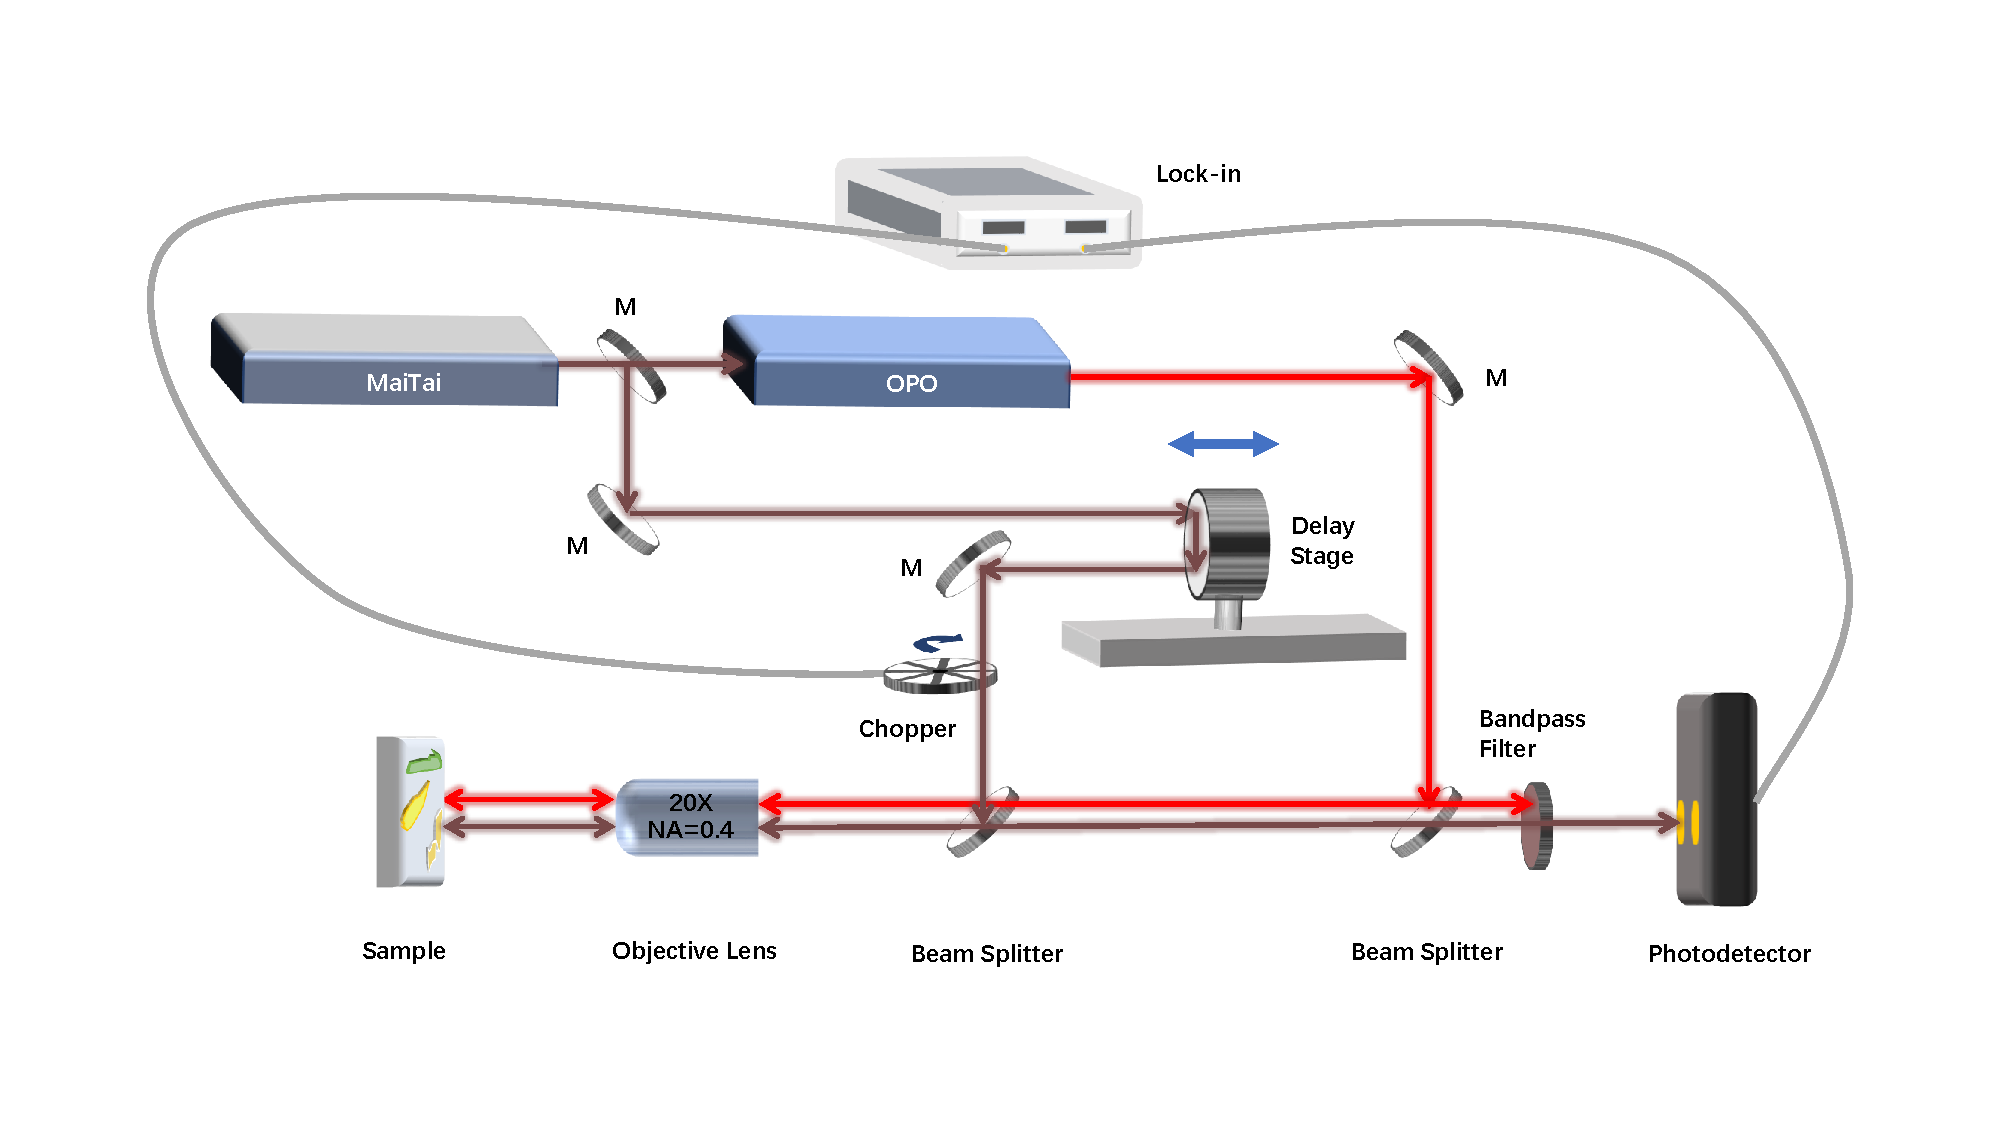
\includegraphics[width=\linewidth]{setup.pdf}
  \caption{Schematics of the transient absorption microscopy.}
    \label{fig:setup}
\end{figure}


%%%%%%%%%%%%%%%%%%%%%%%%%%%%%%%%%%%%%%%%%%%%%%%%%%%%%%%%%%%%%%%%%%%%%
%% The "Acknowledgement" section can be given in all manuscript
%% classes.  This should be given within the "acknowledgement"
%% environment, which will make the correct section or running title.
%%%%%%%%%%%%%%%%%%%%%%%%%%%%%%%%%%%%%%%%%%%%%%%%%%%%%%%%%%%%%%%%%%%%%
\begin{acknowledgement}

The authors thank Chong Wang from Beijing Institute of Technology for his help on the measurements of polarized raman microscope. J.H. is grateful to National Natural Science Foundation of China (61905010), Beijing Municipal Natural Science Foundation (4222073) and the Fundamental Research Funds for the Central Universities (buctrc202003) for financial aid. C.W. would like to thank the Fundamental Research Funds for the Central Universities (buctrc202122) for financial support. Finally, Y.W. appreciates the finical support from National Natural Science Foundation of China (61875236, 61975007) and Beijing Natural Science Foundation of China (Z190006).

\end{acknowledgement}


%%%%%%%%%%%%%%%%%%%%%%%%%%%%%%%%%%%%%%%%%%%%%%%%%%%%%%%%%%%%%%%%%%%%%
%% The appropriate \bibliography command should be placed here.
%% Notice that the class file automatically sets \bibliographystyle
%% and also names the section correctly.
%%%%%%%%%%%%%%%%%%%%%%%%%%%%%%%%%%%%%%%%%%%%%%%%%%%%%%%%%%%%%%%%%%%%%
\bibliography{achemso-demo}

\end{document}
